\documentclass{beamer}

\usepackage[utf8]{inputenc}
\usepackage[T1]{fontenc}
\usepackage[german]{babel}
\usepackage{graphicx} % Bilder
\usepackage{wrapfig} % Umflussbilder
\usepackage{multicol} % Multiple columns
\usepackage{minted} % Haskell source code
\usepackage{framed} % Frames around source code
\usepackage[framemethod=tikz]{mdframed} % Frames

\mdfdefinestyle{fancy}{
  roundcorner=5pt,
  linewidth=4pt,
  linecolor=red!80,
  backgroundcolor=red!20
}
\newmdenv[style=fancy]{important}

% Stuff for Beamer
\beamertemplatenavigationsymbolsempty
\usetheme{Madrid}

\begin{document}

%  \usebackgroundtemplate{\includegraphics[width=\paperwidth,height=\paperheight]{1.jpg}} 
  
%----------------------------------------------------------------------------------------  

  \begin{frame}
  \begin{center}
    \Huge\textbf{Intermediate Functional Programming in Haskell}\\ \bigskip
    \LARGE Universität Bielefeld, Sommersemester 2015\\ \bigskip
    \large Jonas Betzendahl \& Stefan Dresselhaus
    \end{center}
  \end{frame}

%----------------------------------------------------------------------------------------  
  
\begin{frame}
\begin{center}
	\Large\textbf{\underline{Überblick für Heute:}}\\ \bigskip\bigskip\normalsize
	
	Organisatorisches\\\bigskip
	Tools \& Ressourcen\\\bigskip
	Funktionale Programmierung 101\\\bigskip
	Haskell Crash-Kurs
    \end{center}
\end{frame}

%----------------------------------------------------------------------------------------  
  
  \begin{frame}

    \begin{center}
    \Large\textbf{Orga-Krams}
    \end{center}
  \end{frame}

%----------------------------------------------------------------------------------------  
  
  \begin{frame}
    \begin{center}
    \Large\textbf{Orga-Krams (1): Veranstaltungen}\\ \bigskip \normalsize
    Es gibt Vorlesungen (\$wochentag1, AA - BB Uhr in \$Raum1)\\
    und Übungen (\$wochentag2, CC - DD Uhr in \$Raum2).\bigskip

	Die Vorlesungen starten mit einem eher praktisch orientierten Abschnitt ab Heute gefolgt in der zweiten Semesterhälfte von einem eher theoretischen Teil.\bigskip
	
	Teilnahme an den Übungen ist nicht verpflichtend, aber wahrscheinlich für euch von großem Vorteil.  
    \end{center}
  \end{frame}
  
%----------------------------------------------------------------------------------------  
  
  \begin{frame}
    \begin{center}
    \Large\textbf{Orga-Krams (2): Input / Output}\\ \bigskip \normalsize
    
    Für das Modul gibt es 5 (echte) Leistungspunkte\\
    Als Leistung müsst ihr ein kleines Programmierprojekt abschließen.
    Details dazu gibt es in der Übung\bigskip
    
    Wegen bürokratischer Hürden können die Leistungspunkte nur in der \emph{individuellen} Ergänzung eingebracht werden. Nicht in Wahlpflichtbereichen und auch nicht in der strukturierten Ergänzung.
    \end{center}
  \end{frame}
  
%----------------------------------------------------------------------------------------  
  
  \begin{frame}
    \begin{center}
    \Large\textbf{Orga-Krams (3): Personenkult}\\ \bigskip \normalsize

	Wir, das sind Jonas Betzendahl und Stefan Dresselhaus.\\
	Mailadressen: \texttt{\{jbetzend,sdressel\}@techfak\dots}\\ \bigskip
	Wir sind zwei Masterstudenten an der TechFak, die ihren Wunsch nach mehr und besserer Lehre zu funktionaler Programmierung und Haskell hier in Bielefeld jetzt selbst in die Hand nehmen. \bigskip    
    
    Formal verantwortlich ist Dr. Alexander Sczyrba (\texttt{asczyrba@techfak\dots}). Er ist eure Anlaufstelle für Fragen im Kontext der Fakultät und Beschwerden zu uns.
    \end{center}
  \end{frame}
  
%----------------------------------------------------------------------------------------  
  
  \begin{frame}
    \begin{center}
	\Large\textbf{Orga-Krams (4): Material von uns für euch}\\ \bigskip \normalsize
	Alle Übungsblätter, Foliensätze, Beispiele, Vorlagen und sonstige Unterlagen findet ihr entweder im ekVV oder auf der Website dieser Veranstaltung. Die URL ist:
	
	\bigskip\texttt{www.dieseurlmussnochersetztwerden.de}\bigskip
	
	Audio/Video-Mitschnitte findet ihr ebenfalls im Web und zwar auf folgender Seite:
	
	\bigskip\texttt{www.irgendwiesowaswieunirekorder.de}\bigskip
	
	Login: Login, Passwort: 123456
    \end{center}
  \end{frame}
  
%----------------------------------------------------------------------------------------  
  
  \begin{frame}

    \begin{center}
    \Large\textbf{Tools und Ressourcen}
    \end{center}
  \end{frame}
  
%----------------------------------------------------------------------------------------  
  
  \begin{frame}
    \begin{center}
    \Large\textbf{T \& R (1): Haskell / GHC}\\ \bigskip \normalsize
    
    Um auf euren eigenen Rechnern Haskell sinnvoll benutzen zu können benötigt ihr den \texttt{Glasgow Haskell Compiler} (GHC). \bigskip
    
    Der GHC und viele nützliche Dinge mehr sind alle im Rundum-Glücklich-Paket genannt \emph{Haskell Platform} enthalten. Die gibt es für Linux, Mac, BSD und Windows unter folgender URL:
    
    \bigskip\texttt{https://www.haskell.org/platform/}\smallskip
    
    \begin{important}
    \textbf{Wichtig:}\\ Der Interpreter \texttt{Hugs} wird von uns explizit \underline{nicht} unterstützt.
    \end{important}
    \end{center}
  \end{frame}
  
%----------------------------------------------------------------------------------------  
  
  \begin{frame}
    \begin{center}
    \Large\textbf{T \& R (2): GHCi}\\ \bigskip \normalsize
    
    Die mitgelieferte interaktive Umgebung des GHC heißt GHCi.\\\bigskip
    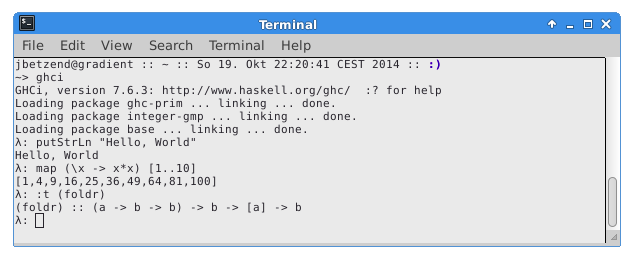
\includegraphics[scale=0.4]{ghci_example.png} 
    
    \bigskip Der GHCi stellt ein REPL (Read - Evaluate - Print - Loop) bereit, die beim Entwickeln \emph{sehr} nützlich sein kann (ähnlich zu \texttt{Hugs}). Mehr dazu in den Übungen.
    \end{center}
  \end{frame}
  
  %----------------------------------------------------------------------------------------  
  
  \begin{frame}
    \begin{center}
    \Large\textbf{T \& R (3): Hackage}\\ \bigskip \normalsize
    Dieser Tage gibt es eine Vielzahl an nützlichen und mächtigen Bibliotheken für Haskell. Zu Hause sind die meisten davon auf \emph{Hackage}: \\ \bigskip \texttt{https://hackage.haskell.org/} \\ \bigskip
    Auf Hackage findet ihr übersichtliche Zusammenfassungen der Bibliotheken, detaillierte Auflistungen der exportierten Funktionen und Datentypen und direkte Links zu den jeweiligen Implementationen (!).
    \end{center}
  \end{frame}
  
%----------------------------------------------------------------------------------------  
  
  \begin{frame}
    \begin{center}
    \Large\textbf{T \& R (4): cabal}\\ \bigskip \normalsize
    Ebenfalls in der \emph{Haskell Platform} enthalten ist \texttt{cabal}, Haskells eigenes Paket-Management-System. \texttt{cabal} erlaubt es euch, einfach via Terminal Bibliotheken von Hackage lokal (!) und im Zweifelsfall auch problemlos in einer Sandbox zu installieren. \texttt{cabal} ist außerdem ein Build-System, kann Test-Suites ausführen und und und. Aber dazu im Zweifelsfall später mehr.\bigskip
    
    Das folgende Beispiel installiert \texttt{lens}, eine Bibliothek die uns im Lauf der Vorlesung noch begegnen wird:\bigskip
   
    \texttt{\$ cabal update \&\& cabal install lens}
    
    
    \end{center}
  \end{frame}
  
%----------------------------------------------------------------------------------------  
  
  \begin{frame}
    \begin{center}
    \Large\textbf{T \& R (5): LYAHFGG}\\ \bigskip \normalsize
    \begin{multicols}{2}
    
	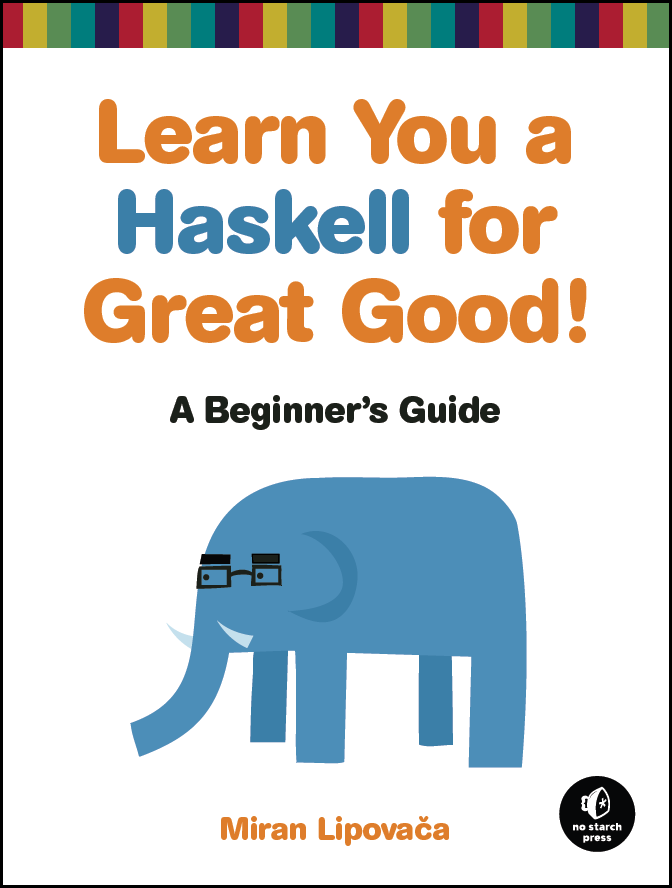
\includegraphics[scale=0.15]{lyah.png} 
	
	\columnbreak    
    Das Buch \glqq Learn You A Haskell\grqq\ ist die beste$^{™}$ Ressource um Haskell zu lernen. Es ist verständlich und locker geschrieben und berühmt für gute Erklärungen.\bigskip
   
    Ihr findet es online frei und kostenlos verfügbar hier:
    
    \texttt{http://learnyouahaskell.com/}
    \end{multicols}
    \end{center}
  \end{frame}
  
%----------------------------------------------------------------------------------------  
  
  \begin{frame}
    \begin{center}
    \Large\textbf{T \& R (6): Hoogle}\\ \bigskip \normalsize
    \emph{Hoogle} ist eine Haskell-API-Suchmaschine, die es möglich macht, nach Funktionen zu suchen, ihren Typen angibt und zeigt, welche Imports nötig sind.\\ Ein besonders nützliches Feature ist, dass es auch möglich ist, nach Typsignaturen zu suchen und darauf passende Antworten zu erhalten.\\ \bigskip
    Die URL lautet: \texttt{http://www.haskell.org/hoogle/}
    \end{center}
  \end{frame}
  
%----------------------------------------------------------------------------------------  
  
  \begin{frame}
    \begin{center}
    \Large\textbf{T \& R (7): Community}\\ \bigskip \normalsize
    Die Haskell-Community ist jenseits von dedizierten Mailingslisten hauptsächlich auf Reddit (\texttt{http://www.reddit.com/r/haskell}) und im IRC (\texttt{\#haskell} auf Freenode) zu finden. Sie gilt als sehr offen, hilfreich und anfängerfreundlich.\\\bigskip
    Als Illustration dazu ein inzwischen berühmt gewordener Ausschnitt aus dem IRC:
    \end{center}
  \end{frame}
  
%----------------------------------------------------------------------------------------  
  
  \begin{frame}

    \framesubtitle{Community} \small
    \texttt{<xQ> HASKELL IS FOR ***** *****. YOU'RE ALL A BUNCH OF ***** ******}\\
    \texttt{<xQ> JAVASCRIPT FOR LIFE *****}\\
    \pause
    \texttt{\dots}\\
    \texttt{<A> xQ: Do you have any specific questions?}\\
    \texttt{<A> xQ: We'd love to help you make your first steps.}\\
    \pause
    \texttt{<xQ> i just want to get kicked out of a bunch of channels for fun}\\
    \texttt{<A> Have you seen LYAH? It's a very enjoyable book on Haskell. It also has a reputation of being very uplifting.}\\
    \texttt{<xQ> why is no one cooperating with me?}\\
    \pause
    \texttt{\dots}\\
    \texttt{<xQ> what's haskell good for though?}\\
    \texttt{\dots}\\
    \texttt{<xQ> Alright thanks guys, I'll be back later to actually learn some haskell for real}\\
  \end{frame}

%----------------------------------------------------------------------------------------  
  
  \begin{frame}

    \begin{center}
    \Large\textbf{Funktionale Programmierung 101}
    \end{center}
  \end{frame}
  
%----------------------------------------------------------------------------------------  
  
  \begin{frame}
    \begin{center}
    \Large\textbf{FP-101 (1): Definition}\\ \bigskip \normalsize
    
    \textbf{Funktionale Programmierung} ist ein \emph{deklaratives} Programmierparadigma, in dem darauf abgezielt wird, den Programmfluss als Auswertung mehrerer (mathematischer) Funktionen auszudrücken. Dabei wird besonderer Wert darauf gelegt, so genannte \emph{Seiteneffekte} zu vermeiden.

    \end{center}
  \end{frame}
  
%----------------------------------------------------------------------------------------  
  
\begin{frame}[fragile]
    \begin{center}
    \Large\textbf{FP-101 (2): Deklaratives Programmieren}\\ \bigskip \normalsize    
    \end{center}
    
    Im Gegensatz zur imperativen Programmierung gibt der Programmierer nur an, \emph{welche} Werte er errechnet bekommen möchte, nicht jedoch, \emph{wie} sie berechnet werden sollen. Das bleibt der Implementierung der Sprache (dem Compiler) überlassen. 
    
\begin{minted}[size=\footnotesize]{haskell}
triples :: (Int, Int, Int)
triples = [(a,b,c) | a <- [1..10], b <- [1..10], 
                     c <- [1..10], a^2 + b^2 == c^2]
\end{minted}
    
\end{frame}

%----------------------------------------------------------------------------------------  
  
\begin{frame}[fragile]
    \begin{center}
        \Large\textbf{FP-101 (3): Seiteneffekte}\\ \bigskip \normalsize    
    
\begin{minted}{java}
   public int fuenf()
   {
       System.out.println("Seiteneffekt!");
       global_var = null;
       return 5;
   }
\end{minted} 
    \end{center}

Diese zwei Statements haben sehr (!) unterschiedliches Verhalten:    
    
    \mint{java}|return 5 + 5;       // referential transparency|

    \mint{java}|return 5 + fuenf(); // no referential transparency|  

\end{frame}
  
%----------------------------------------------------------------------------------------  
  
\begin{frame}[fragile]
    \begin{center}
     \Large\textbf{FP-101 (4): Higher-Order Functions}\\ \bigskip \normalsize    
    \end{center}
    
    Funktionen mit anderen Funktionen als Parameter.\\
    \texttt{map} z.B. wendet eine Funktion auf alle Elemente einer Liste an. 

\begin{minted}{haskell}
ghci > map (+10) [1..10]
[11,12,13,14,15,16,17,18,19,20]

ghci > map reverse ["abcde", "123", "kayak", "haskell"]
["edcba","321","kayak","lleksah"]
\end{minted}    
    
\end{frame}
  
\end{document}